\subsection{Conceptual Design}

\newpage

\subsubsection{Class Diagram not restructured}

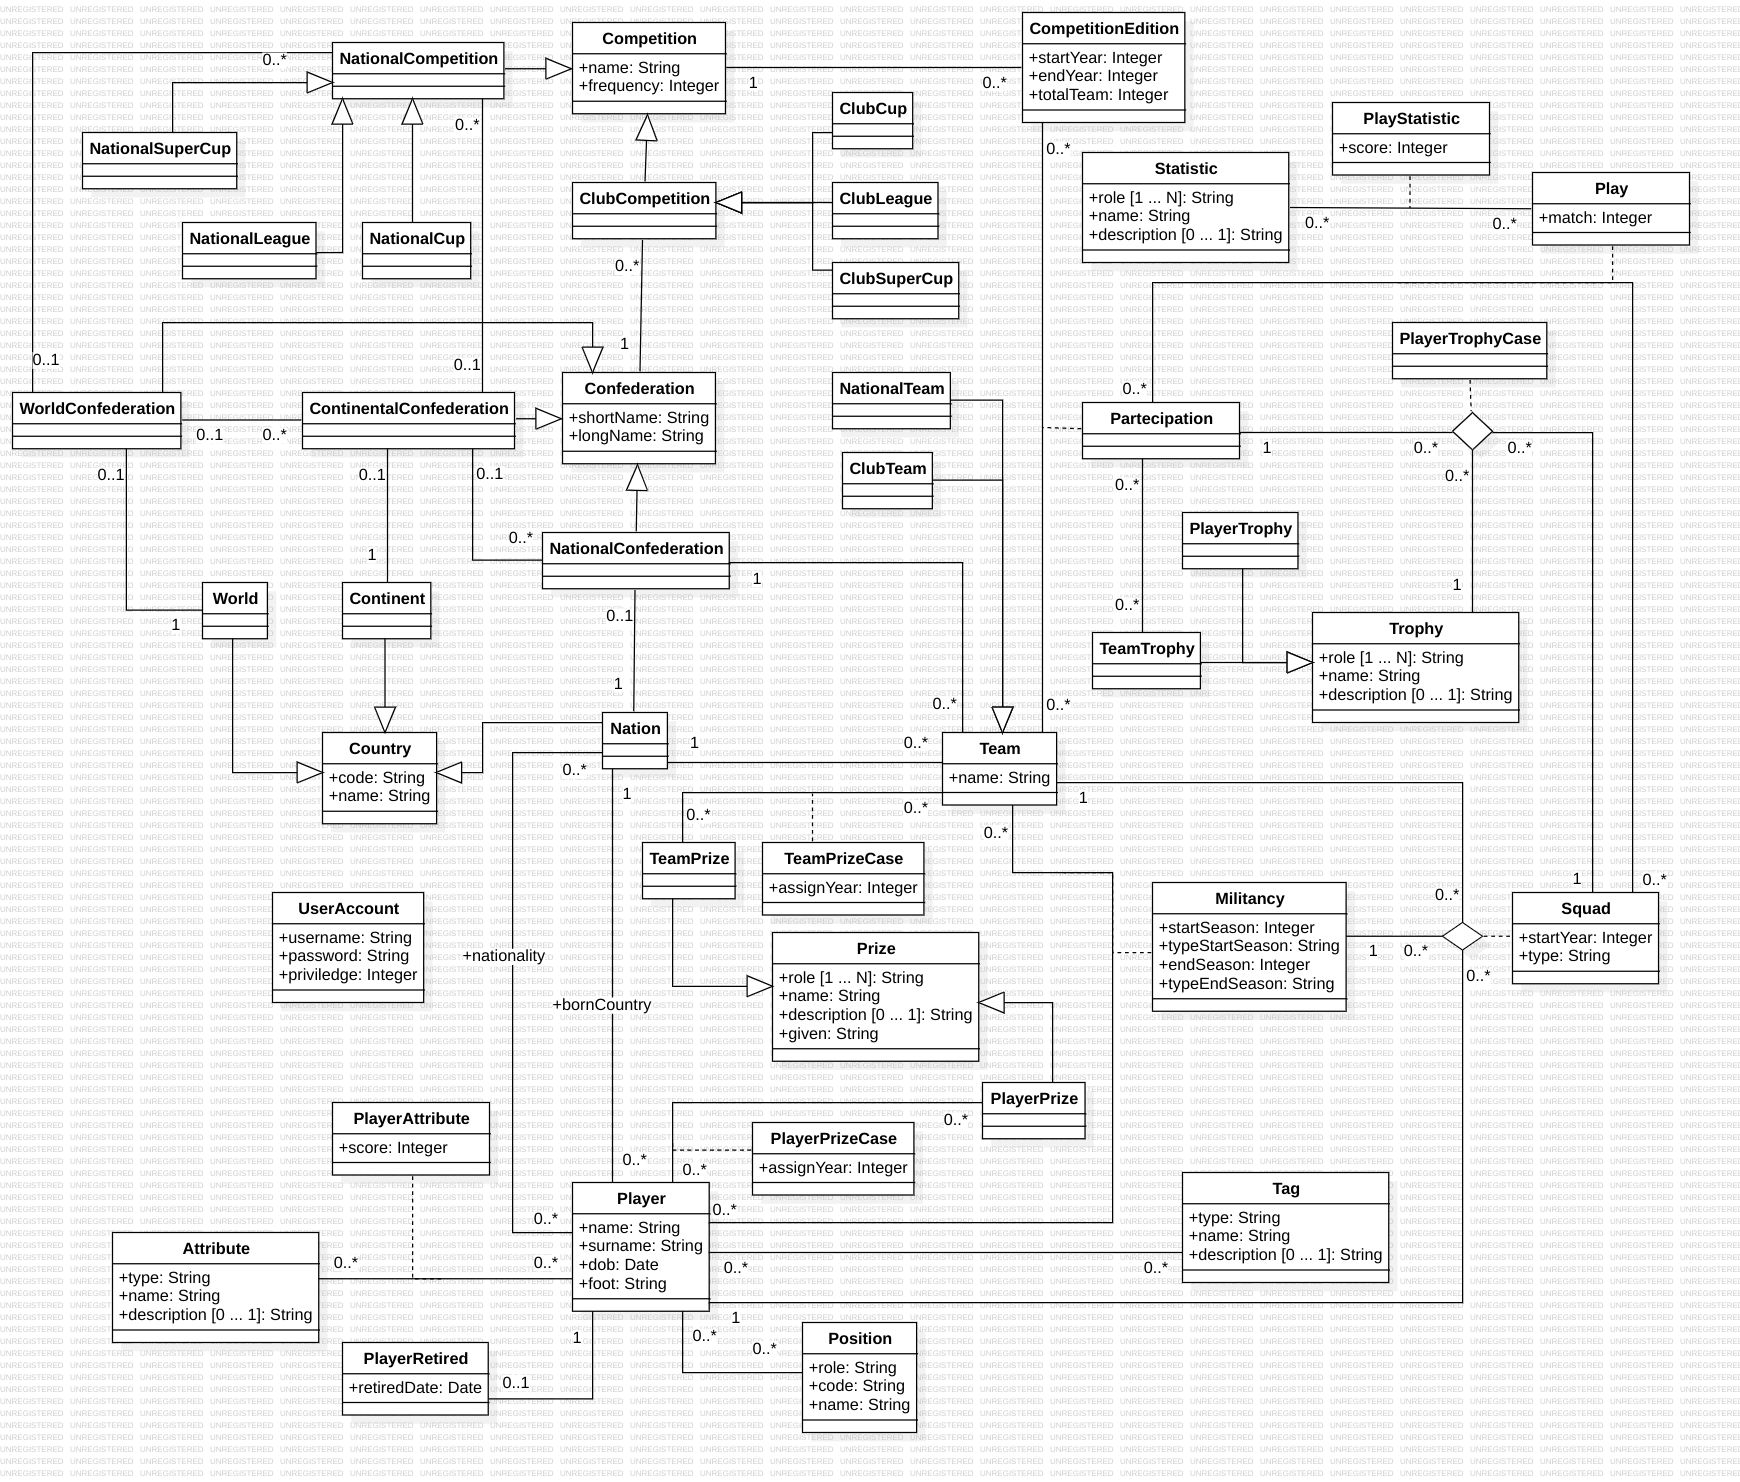
\includegraphics[width=\textwidth]{res/class_diagram_not_restr}
\newpage

\subsubsection{Analysis of the Class Diagram's restructuring}
\newpage
\subsubsection{Restructured Class Diagram}
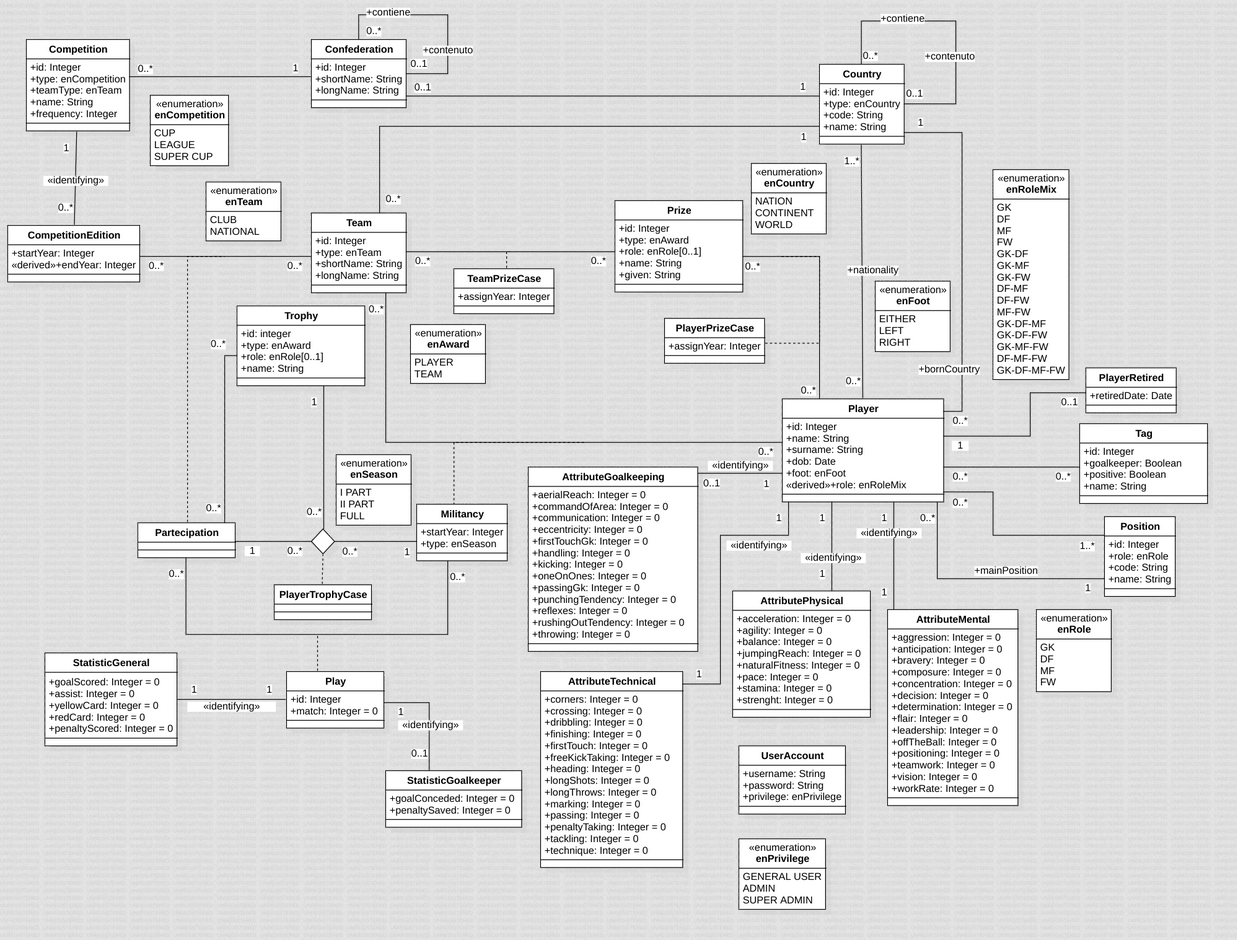
\includegraphics[scale= 0.242]{res/class_diagram_ristr}
\newpage

\subsubsection{Dizionario}

\begin{center}
	\textbf{Dizionario delle Classi}
\end{center}


\begin{tblr}{
    hlines = {0.9pt}, vlines = {0.9pt}, colspec = {X[l]X[l]X[l]}, column{1}= {100pt},
    width = \textwidth, cell{1}{1-3} = {blue!10!white}
}
	{
		Classe
	}
	&
	{
		Descrizione
	}
	&
	{
		Attributo
	}
	\\
	{
		Attribute
	}
	&
	{
		Rappresenta gli attributi di un calciatore.
	}
	&
	{
		\textbf{id}(Integer)[chiave surrogata]:\\Rappresenta
			l'identificativo di un Attributo.\\
		\medskip\textbf{type}(enFeature):\\Rappresenta
			il tipo di un Attributo.\\
		\medskip\textbf{name}(String)[chiave naturale]:
			\\Rappresenta il nome di un Attributo.\\
		\medskip\textbf{description}(String)[parziale]:
			\\Rappresenta la descrizione di un Attributo.
	}
	\\
	{
		Competition
	}
	&
	{
		Rappresenta le competizioni calcistiche.
	}
	&
	{
		\textbf{id}(Integer)[chiave surrogata]:\\Rappresenta
			l'identificativo di una Competizione.\\
		\medskip\textbf{type}(enCompetition):\\Rappresenta
			il tipo di una Competizione.\\
		\medskip\textbf{teamType}(enTeam):\\Rappresenta
			il tipo di squadra che può
			partecipare alla Competizione.\\
		\medskip\textbf{name}(String)[chiave naturale]:
			\\Rappresenta il nome di una Competizione.\\
		\medskip\textbf{frequency}(Integer):\\Rappresenta
			la frequenza di una Competizione.
	}
	\\
	{
		CompetitionEdition
	}
	&
	{
		Rappresenta le edizioni delle competizioni calcistiche.
	}
	&
	{
		\textbf{id}(Integer)[chiave surrogata]:\\Rappresenta
			l'identificativo di un'Edizione.\\
		\medskip\textbf{startYear}(Integer)[chiave parziale]:
			\\Rappresenta l'anno di inizio di un'Edizione.\\
		\medskip\textbf{endYear}(Integer)[chiave parziale]:
			\\Rappresenta l'anno di fine di un'Edizione.\\
		\medskip\textbf{totalTeam}(Integer):\\Rappresenta
			il numero di team che partecipano in un'Edizione.
	}
	\\
	{
		Confederation
	}
	&
	{
	Rappresenta le confederazioni calcistiche.
	}
	& 
	{
		\textbf{id}(Integer)[chiave surrogata]:\\Rappresenta
			l'identificativo di una Confederazione.\\
		\medskip\textbf{shortName}(String):\\Rappresenta
			il nome abbreviato di una Confederazione.\\
		\medskip\textbf{longName}(String)[chiave naturale]:
			\\Rappresenta il nome esteso di una Confederazione.
	}
	\\
\end{tblr}

\begin{tblr}{
    hlines = {0.9pt}, vlines = {0.9pt}, colspec = {X[l]X[l]X[l]}, column{1}= {100pt},
    width = \textwidth
}
	{
		Country
	}
	&
	{
		Rappresenta i paesi in cui si gioca
		ufficialmente a calcio.
	}
	&
	{
		\textbf{id}(Integer)[chiave surrogata]:\\Rappresenta
			l'identificativo di un Paese.\\
		\textbf{type}(enCountry):\\Rappresenta
			il tipo di un Paese.\\
		\medskip\textbf{code}(String)[chiave naturale]:
			\\Rappresenta il codice ISO 3166-1 alpha-3
			di un Paese.\\
		\medskip\textbf{name}(String)[chiave naturale]:
			\\Rappresenta il nome di un Paese.
	}
	\\
	{
		Militancy
	}
	&
	{
		Rappresenta le militanze di un
		calciatore in una squadra.
	}
	&
	{
		\textbf{id}(Integer)[chiave surrogata]:\\Rappresenta
			l'identificativo di una Militanza.\\
		\medskip\textbf{dateRange}(daterange):\\Rappresenta
			il periodo di tempo in cui
			un calciatore era nella squadra.
	}
	\\
	{
		MilitancyStatistic
	}
	&
	{
		Rappresenta l'associazione tra
		Militancy e Statistic.\\È una classe associativa.
	}
	& 
	{
		\textbf{score}(Integer)[derivato]:\\Rappresenta
			il valore di una Statistica per
			la Militanza associata.
	}
	\\
	{
		Partecipation
	}
	&
	{
		Rappresenta la partecipazione
		di un Team ad una CompetitionEdition.\\
		È una classe associativa.
	}
	&
	{
	
	}
	\\
	{
		Play
	}
	&
	{
		Rappresenta l'associazione tra
		Partecipation e PlayerPosition.\\
		È una classe associativa.
	}
	&
	{
		\textbf{id}(Integer)[chiave surrogata]:\\Rappresenta
			l'identificativo di un Play.
	}
	\\
	{
		PlayStatistic
	}
	&
	{	
		Rappresenta l'associazione tra Play e Statistic.\\
		È una classe associativa.
	}
	&
	{
		\textbf{score}(Integer):\\Rappresenta
			il valore di una Statistica per il Play associato.
	}
	\\
	{
		Player
	}
	&
	{
		Rappresenta i calciatori.
	}
	&
	{
		\textbf{id}(Integer)[chiave surrogata]:\\Rappresenta
			l'identificativo di un Calciatore.\\
		\medskip\textbf{name}(String):\\Rappresenta
			il nome di un Calciatore.\\
		\medskip\textbf{surname}(String):\\Rappresenta
			il cognome di un Calciatore.\\
		\medskip\textbf{dob}(Date):\\Rappresenta
			la data di nascita.\\
		\medskip\textbf{foot}(enFoot):\\Rappresenta
			il piede preferito di un Calciatore.\\
		\medskip\textbf{careerTime}(daterange):\\Rappresenta
			l'intervallo di tempo tra la data di debutto
			e la data di ritiro di un Calciatore.
	}
	\\
	{
		PlayerAttribute
	}
	&
	{
		Rappresenta l'associazione tra Player e Attribute.\\
		È una classe associativa.
	}
	&
	{
		\textbf{score}(Integer):\\Rappresenta
			il valore di un Attributo associato al Calciatore.
	}
	\\
\end{tblr}

\begin{tblr}{
    hlines = {0.9pt}, vlines = {0.9pt}, colspec = {X[l]X[l]X[l]}, column{1}= {100pt},
    width = \textwidth
}
	{
		PlayerPosition
	}
	&
	{
		Rappresenta l'associazione tra Player e Position.\\
		È una classe associativa.
	}
	&
	{
		\textbf{match}(Integer)[derivato]:\\Rappresenta
			il numero di partite che un Calciatore gioca
			in una determinata Posizione.
	}
	\\
	{
		PlayerPrizeCase
	}
	&
	{
		Rappresenta la bacheca dei premi del calciatore.
	}
	&
	{
		\textbf{assignYear}(Integer):\\Rappresenta
			l'anno di assegnazione di un Premio.
	}
	\\
	{
		PlayerTrophyCase
	}
	&
	{
		Rappresenta la bacheca dei trofei di un calciatore.
	}
	&
	{
	
	}
	\\
	{
		Position
	}
	&
	{
		Rappresenta le posizioni di gioco di un Calciatore.
	}
	&
	{
		\textbf{id}(Integer)[chiave surrogata]:\\Rappresenta
			l'identificativo di una Posizione.\\
		\medskip\textbf{role}(enRole):\\Rappresenta
			il ruolo associato ad una Posizione.\\
		\medskip\textbf{code}(String)[chiave naturale]:
			\\Rappresenta il nome abbreviato di una Posizione.\\
		\medskip\textbf{name}(String)[chiave naturale]:
			\\Rappresenta il nome di una Posizione.
	}
	\\
	{
		Prize
	}
	&
	{
		Rappresenta i premi calcistici.
	}
	&
	{
		\textbf{id}(Integer)[chiave surrogata]:\\Rappresenta
			l'identificativo del Premio.\\
		\medskip\textbf{type}(enAward):\\Rappresenta
			il tipo del Premio.\\
		\medskip\textbf{name}(String)[chiave naturale]:
			\\Rappresenta il nome del Premio.\\
		\medskip\textbf{description}(String)[parziale]:
			\\Rappresenta la descrizione del Premio.\\
		\medskip\textbf{given}(String):\\Rappresenta
			il nome della società calcistica
			che conferisce il Premio.
	}
	\\
	{
		Statistic
	}
	&
	{
		Rappresenta le statistiche di un calciatore.
	}
	&
	{
		\textbf{id}(Integer)[chiave surrogata]:\\Rappresenta
			l'identificativo della Statistica.\\
		\medskip\textbf{role}(enRoleMix):\\Rappresenta
			i ruoli associati alla Statistica.\\
		\medskip\textbf{name}(String):\\Rappresenta
			il nome della Statistica.\\
		\medskip\textbf{description}(String)[parziale]:
			\\Rappresenta la descrizione della Statistica.
	}
	\\
\end{tblr}


\begin{tblr}{
    hlines = {0.9pt}, vlines = {0.9pt}, colspec = {X[l]X[l]X[l]}, column{1}= {100pt},
    width = \textwidth
}
	{
		Tag
	}
	&
	{
		Rappresenta i tag di un calciatore.
	}
	&
	{
		\textbf{id}(Integer)[chiave surrogata]:\\Rappresenta
			l'identificativo del Tag.\\
		\medskip\textbf{type}(enFeature):\\Rappresenta
			il tipo del Tag.\\
		\medskip\textbf{name}(String)[chiave naturale]:
			\\Rappresenta il nome del Tag.\\
		\medskip\textbf{description}(String)[parziale]:
			\\Rappresenta la descrizione del Tag.
	}
	\\
	{
		Team
	}
	&
	{
		Rappresenta le squadre di calcio.
	}
	&
	{
		\textbf{id}(Integer)[chiave surrogata]:\\Rappresenta
			l'identificativo della Squadra.\\
		\medskip\textbf{type}(enTeam):\\Rappresenta
			il tipo della Squadra.\\
		\medskip\textbf{name}(String)[chiave naturale]:
			\\Rappresenta il nome della Squadra.
	}
	\\
	{
		TeamPrizeCase
	}
	&
	{
		Rappresenta la bacheca dei premi della squadra.
	}
	&
	{
		\textbf{assignYear}(Integer):\\Rappresenta
			l'anno di assegnazione di un Premio.
	}
	\\
	{
		Trophy
	}
	&
	{
		Rappresenta i trofei calcistici.
	}
	&
	{
		\textbf{id}(Integer)[chiave surrogata]:\\Rappresenta
			l'identificativo del Trofeo.\\
		\medskip\textbf{type}(enAward):\\Rappresenta
			il tipo del Trofeo.\\
		\medskip\textbf{name}(String)[chiave naturale]:
			\\Rappresenta il nome del Trofeo.\\
		\medskip\textbf{description}(String)[parziale]:
			\\Rappresenta la descrizione del Trofeo.\\
	}
	\\
	{
		UserAccount
	}
	&
	{
		Rappresenta gli utenti dell'applicativo.
	}
	&
	{
		\textbf{username}(String)[chiave naturale]:\\Rappresenta
			l'username dell'Account dell'Utente.\\
		\medskip\textbf{password}(String):\\Rappresenta
			la password dell'Account dell'Utente.\\
		\medskip\textbf{priviledge}(Integer):\\Rappresenta
			i privilegi dell'Account dell'Utente.
	}
	\\
\end{tblr}

\newpage

\begin{center}
	\textbf{Dizionario delle Associazioni}
\end{center}



\begin{tblr}{
    hlines = {0.9pt}, vlines = {0.9pt}, colspec = {X[l]X[l]X[l]}, column{1}= {100pt},
    width = \textwidth, cell{1}{1-3} = {blue!10!white}
}

	{
		Nome
	}
	&
	{
		Descrizione
	}
	&
	{
		Classi in Relazione
	}
	\\
	{
		Nationality
	}
	&
	{
		Esprime le nazionalità di un calciatore.\\
		È una relazione N a N.
	}
	&
	{
		\textbf{Country [0 ... *]}:\\Indica che
			uno stesso paese può essere associato a più
			calciatore.\\
		\medskip\textbf{Player [0 ... *]}:\\Indica che
			un calciatore può avere più nazionalità.
	}
	\\
	{
		bornCountry	
	}
	&
	{
		Esprime il paese di nascita di un calciatore.\\
		È una relazione 1 a N.
	}
	&
	{
		\textbf{Country [0 ... *]}:\\Indica che
			un paese può essere il paese di nascita
			di più calciatori.\\
		\medskip\textbf{Player [1]}:\\Indica che
			un calciatore ha uno e un solo paese di nascita.
	}
	\\
	{
		Player-PlayerAttribute
	}
	&
	{
		Esprime il valore degli attributi di un calciatore.\\
		È una relazione 1 a N.
	}
	&
	{
		\textbf{Player [0 ... *]}:\\Indica che un Calciatore
			può aver zero o più valori di Attributi associati.\\
		\medskip\textbf{PlayerAttribute [1]}:\\Indica che 
			un valore di un Attributo deve essere associato
			ad uno e un solo Calciatore.
	}
	\\
	{
		PlayerAttribute-Attribute
	}
	&
	{
		Esprime a quale attributo si riferisce
		PlayerAttribute.\\È una relazione 1 a N.
	}
	&
	{
		\textbf{PlayerAttribute [1]}:\\Indica che un valore
			di PlayerAttribute è associato ad uno e un solo
			Attributo.\\
		\medskip\textbf{Attribute [0 ... *]}:\\Indica che un
			Attributo può avere più valori associati.
	}
	\\
	{
		Player-Tag
	}
	&
	{
		Esprime i Tag associati ad un Calciatore.\\
		È una relazione N a N.
	}
	&
	{
		\textbf{Player [0 ... *]}:\\Indica che un Calciatore
			può avere più Tag associati.\\
		\medskip\textbf{Tag [0 ... *]}\\Indica che
			uno stesso Tag può essere associato a
			più Calciatori.
	}
	\\
	{
		Player - PlayerTrophyCase
	}
	&
	{
		Esprime i trofei associati ad un calciatore.\\
		È una relazione 1 a N.
	}	
	&
	{
		\textbf{Player [0 ... *]}:\\Indica che un Calciatore
			può avere più Trofei associati.\\
		\medskip\textbf{PlayerTrophyCase [1]}:\\Indica che una
			bacheca si può riferire ad uno e un solo Calciatore.
	}
	\\
	{
		PlayerTrophyCase - Trophy
	}
	&
	{
		Esprime i trofei associati ad una bacheca.\\
		È una relazione 1 a N.
	}
	&
	{
		\textbf{PlayerTrophyCase [1]}:\\Indica che una bacheca
			si può riferire ad uno e un solo Trofeo.\\
		\medskip\textbf{Trophy [0 ... *]}:\\Indica che
			un Trofeo può avere più bacheche associate.
	}
	\\
	{
		PlayerTrophyCase - Partecipation
	}
	&
	{
		Esprime le partecipazioni di una squadra
		ad una competizione edizione associate
		ad una bacheca.\\
		È una relazione 1 a N.
	}
	&
	{
		\textbf{PlayerTrophyCase [1]}:\\Indica che una bacheca
			si può riferire ad uno e un sola Partecipazione.
		\medskip\textbf{Partecipation [0 ... *]}:\\Indica che
			una Partecipazione può avere più bacheche associate.
	}
	\\
	{
		Player-PlayerPosition
	}
	&
	{
		Esprime il numero di partite che un Calciatore
		ha fatto in una certa posizione.\\
		È una relazione 1 a N.
		
	}
	&
	{
		\textbf{Player [0 ... *]}:\\Indica che un Calciatore
			può avere più posizioni di gioco associate.\\
		\medskip\textbf{PlayerPosition [1]}:\\Indica che
			il numero di partite di una posizione di gioco si
			può riferire ad uno e un solo Calciatore.
	}
	\\
	{
		PlayerPosition-Position
	}
	&
	{
		Esprime a quale posizione è associato
		il numero di partite di un Calciatore.\\
		È una relazione 1 a N.
	}
	&
	{
		\textbf{PlayerPosition [1]}:\\Indica che il numero
			di partite di una posizione di gioco si può riferire
			ad una e una sola posizione.\\
		\medskip\textbf{Position [0 ... *]}:\\Indica che
			una Posizione può avere più calciatori associati.
	}
	\\
	{
		Player-Militancy
	}
	&
	{
		Esprime le Militanze associate ad un Calciatore.\\
		È una relazione 1 a N.
	}
	&
	{
		\textbf{Player [0 ... *]}:\\Indica che il Calciatore
			può avere più Militanze associate.\\
		\medskip\textbf{Militancy [1]}:\\Indica che
			una Militanza si può riferire ad uno
			e un solo Calciatore.
	}
	\\
	{
		Militancy-Team
	}
	&
	{
		Esprime a quale Squadra una Militanza è associata.\\
		È una relazione 1 a N.
	}
	&
	{
		\textbf{Militancy [1]}:\\Indica che una Militanza
			si può riferire ad una e una sola Squadra.\\
		\medskip\textbf{Team [0 ... *}:\\Indica che una Squadra
			può avere più Militanze associate.
	}
	\\
	{
		Player-PlayerPrizeCase
	}
	&
	{
		Esprime i premi associati ad un Calciatore
		nella Bacheca.\\È una relazione 1 a N.
	}
	&
	{
		\textbf{Player [0 ... *]}:\\Indica che un Calciatore
			può avere più premi associati in una Bacheca.
		\medskip\textbf{PlayerPrizeCase [1]}:\\Indica che una
			Bacheca si può riferire ad un e un solo Calciatore.
	}
	\\
	{
		PlayerPrizeCase-Prize
	}
	&
	{
		Esprime i Premi ai quali è associata una Bacheca.\\
		È una relazione 1 a N.
	}
	&
	{
		\textbf{PlayerPrizeCase [1]}:\\Indica che una Bacheca
			si può riferire ad un e un solo Premio.\\
		\medskip\textbf{Prize [0 ... *]}:\\Indica che un Premio
			può avere più Bacheche associate.
	}
	\\
	{
		Team-Country
	}
	&
	{
		Esprime la nazionalità di una Squadra.\\
		È una relazione 1 a N.
	}
	&
	{
		\textbf{Team [1]}:\\Indica che una Squadra si riferisce
			ad un e un solo paese.\\
		\medskip\textbf{Country [0 ... *]}:\\Indica che un Paese
			può avere più Squadre associate.
	}
	\\
	{
		Team-Confederation
	}
	&
	{
		Esprime la Confederazione di cui una Squadra è membra.\\
		È una relazione 1 a N.
	}
	&
	{
		\textbf{Team [1]}:\\Indica che una Squadra si riferisce
			ad una e una sola Confederazione.\\
		\medskip\textbf{Confederation [0 ... *]}:\\Indica che
			una Confederazione può avere più Squadre associate.
	}
	\\
	{
		Team-Partecipation	
	}
	&
	{
		Esprime le edizioni delle Competizioni a cui una Squadra
		Partecipa.\\È una relazione 1 a N.
	}
	&
	{
		\textbf{Team [0 ... *]}:\\Indica che una Squadra può
			partecipare a più Competizioni Edizioni.\\
		\medskip\textbf{Partecipation [1]}:\\Indica che una
			Partecipazione può riferirsi ad una e una sola
			Squadra.
	}
	\\
	{
		Partecipation-CompetitionEdition
	}
	&
	{
		Esprime a quali Edizioni di una Competizione una
		Partecipazione di una Squadra si riferisce.\\
		È una relazione 1 a N.
	}
	&
	{
		\textbf{Partecipation [1]}:\\Indica che
			una Partecipazione può riferirsi ad una e una sola
			Edizione di una Competizione.\\
		\medskip\textbf{CompetitionEdition [0 ... *]}:\\Indica
			che una Edizione di una Competizione può avere più
			Partecipazioni associate.
	}
	\\
	{
		Team-TeamPrizeCase
	}
	&
	{
		Esprime i premi associati ad una Squadra
		in una Bacheca.\\È una relazione 1 a N.
	}
	&
	{
		\textbf{Team [0 ... *]}:\\Indica che una Squadra
			può avere più premi associati in una Bacheca.\\
		\medskip\textbf{TeamPrizeCase [1]}:\\Indica che una
			Bacheca si può riferire ad una e una sola Squadra.
	}
	\\
	{
		TeamPrizeCase-Prize	
	}
	&
	{
		Esprime i Premi ai quali è associata una Bacheca.\\
		È una relazione 1 a N.
	}
	&
	{
		\textbf{TeamPrizeCase [1]}:\\Indica che una Bacheca
			si può riferire ad un e un solo Premio.\\
		\medskip\textbf{Prize [0 ... *]}:\\Indica che un Premio
			può avere più Bacheche associate.
	}
	\\
	{
		Confederation-Country
	}
	&
	{
		Esprime l'appartenza di una Confederazione
		ad un unico Paese e viceversa.\\È una relazione 1 a 1.
	}
	&
	{
		\textbf{Confederation [1]}:\\Indica che
			una Confederazione si può riferire
			ad un e un solo Paese.\\
		\medskip\textbf{Country [1]}:\\Indica che un Paese
			si può riferire ad una e una sola Confederazione.
	}
	\\
	{
		Membro
	}
	&
	{
		Esprime la possibilità di una confederazione di
		avere come membri altre confederazioni, o essere
		membro a sua volta.\\
		È una relazione 1 a N.
	}
	&
	{
		\textbf{Confederation [0 ... 1]} ruolo (contenuto):\\
			Indica che una Confederazione può o non può essere
			membra di un'altra Confederazione.
		\medskip\textbf{Confederation [0 ... *]}
			ruolo (contiene):\\
			Indica che una Confederazione può avere più
			Confederazioni come membri.
	}
	\\
	{
		Confederation-Competition
	}
	&
	{
		Esprime la capacità di una Confederazione di creare
		Competizioni.\\È una relazione 1 a N.
	}
	&
	{
		\textbf{Confederation [0 ... *]}:\\Indica che una
			Confederazione può creare più Competizioni.
		\medskip\textbf{Competition [1]}:\\Indica che una
			Competizione si riferisce ad una e una sola
			Confederazione.
	}
	\\
\end{tblr}